\paragraph{QuizziPedia::Front-End::Controllers::MenuBarController}
\begin{figure} [ht]
	\centering
	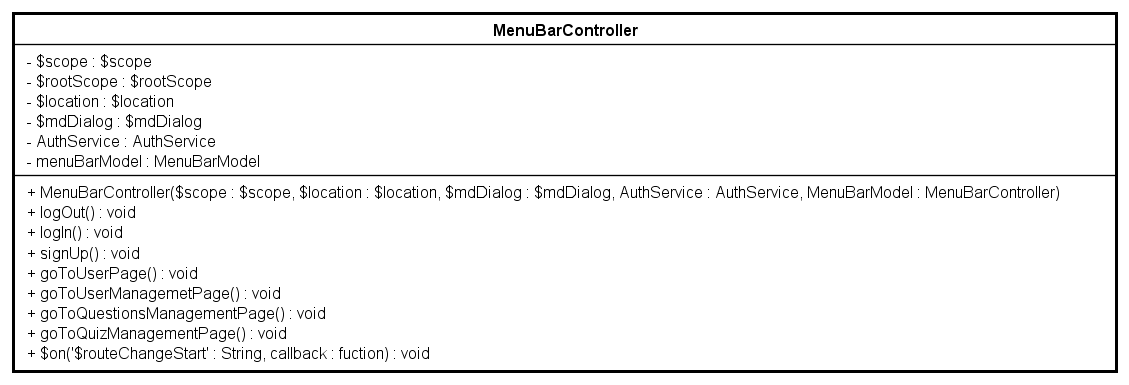
\includegraphics[scale=0.45]{UML/Classi/Front-End/QuizziPedia_Front-end_Controller_MenuBarController.png}
	\caption{QuizziPedia::Front-End::Controllers::MenuBarController}
\end{figure} \FloatBarrier
\begin{itemize}
	\item \textbf{Descrizione}: questa classe permette di gestire il menù fisso per ogni pagina;
	\item \textbf{Utilizzo}: fornisce le funzionalità per aggiornare, a seconda della pagina, il contenuto del menù;
	\item \textbf{Relazione con altre classi}:
	\begin{itemize}
		\item \textit{IN} \texttt{MenuBarModelView}: classe di tipo modelview la cui istanziazione è contenuta all'interno della variabile di ambiente \$scope di \textit{Angular.js\ped{G}}. All'interno di essa sono presenti le variabili e i metodi necessari per il \textit{Two-Way Data-Binding\ped{G}} tra la directive \texttt{MenuBarDirective} e il controller \texttt{MenuBarController}. Rappresenta il menù, presente in ogni pagina dell'applicazione, generato in base agli oggetti passati nello \$scope. Fornisce un pulsante per ogni oggetto ricevuto come parametro, ogni pulsante viene rappresentato con un’icona e con un testo. Al click di un pulsante viene invocata la funzione ad esso associata; 
		\item \textit{IN} \texttt{AuthService}: questa classe permette di gestire la registrazione e l'autenticazione di un utente;
		\item \textit{IN} \texttt{MenuBarModel}: questa classe rappresenta la classe che contiene le informazioni per la giusta visualizzazione della barra.
	\end{itemize}
	\item \textbf{Attributi}:
	\begin{itemize}
		\item \texttt{-} \texttt{\$scope: \$scope} \\
		Campo dati contenente un riferimento all’oggetto \$scope creato da \textit{Angular\ped{G}}, viene utilizzato come mezzo di comunicazione tra il controller e la view. Contiene gli oggetti che definiscono il model dell’applicazione;
		\item \texttt{-} \texttt{\$rootScope: \$rootScope} \\
		Campo dati contenente il riferimento all'oggetto globale \$rootScope creato da \textit{Angular\ped{G}};
		\item \texttt{-} \texttt{\$location: \$location} \\
		Campo dati contenente un riferimento al servizio creato da \textit{Angular\ped{G}} che permette di accedere alla barra degli indirizzi del \textit{browser\ped{G}}, i cambiamenti all’URL nella barra degli indirizzi si riflettono in questo oggetto e viceversa; 
		\item \texttt{-} \texttt{\$mdDialog: \$mdDialog} \\
		Campo dati contenente un riferimento al servizio della libreria \textit{Material for Angular\ped{G}} che permette di creare delle componenti a popup;
		\item \texttt{-} \texttt{AuthService: AuthService} \\
		Campo dati contenente un riferimento al servizio che si occupa della gestione delle informazioni legate all’autenticazione;
		\item \texttt{-} \texttt{menuBarModel: MenuBarModel}: \\
		Campo dati contenente un riferimento all'oggetto che contiene le informazioni per la giusta visualizzazione della barra.
	\end{itemize}
	\item \textbf{Metodi}:
	\begin{itemize}
		\item \texttt{+} \texttt{MenuBarController(\$scope: \$scope, \$location: \$location, \$mdDialog: \$mdDialog, AuthService: AuthService, MenuBarModel: MenuBarModel)} \\
		Metodo costruttore della classe; \\
		\textbf{Parametri}:
		\begin{itemize}
			\item \texttt{\$scope: \$scope} \\
			Parametro contenente un riferimento all’oggetto \$scope creato da \textit{Angular\ped{G}}. Viene utilizzato come mezzo di comunicazione tra il controller e la view. Contiene gli oggetti che definiscono il viewmodel e il model dell’applicazione;
			\item \texttt{\$rootScope: \$rootScope} \\
			Campo dati contenente il riferimento all'oggetto globale \$rootScope creato da \textit{Angular\ped{G}};
			\item \texttt{\$location: \$location} \\
			Parametro contenente un riferimento al servizio creato da \textit{Angular\ped{G}} che permette di accedere alla barra degli indirizzi del \textit{browser\ped{G}}, i cambiamenti all’URL nella barra degli indirizzi si riflettono in questo oggetto e viceversa;
			\item \texttt{\$mdDialog: \$mdDialog} \\
			Parametro contenente un riferimento al servizio della libreria \textit{Material for Angular\ped{G}} che permette di creare delle componenti a popup;
			\item \texttt{AuthService: AuthService} \\
			Parametro contenente un riferimento al servizio che si occupa della gestione delle informazioni legate all’autenticazione.  Viene utilizzato il metodo \texttt{logOut} di \$texttt{AuthService} a cui viene passato il parametro \texttt{username};
			\item \texttt{MenuBarModel: MenuBarModel}: \\
			Parametro contenente un riferimento all'oggetto che contiene le informazioni per la giusta visualizzazione della barra.
		\end{itemize}
		\item \texttt{+} \texttt{logOut(): void} \\
		Metodo che richiama il metodo \texttt{logOut} del service \texttt{AuthService} passandogli lo \texttt{username}. Prima di effettuare questa operazione viene mostrato a video un messaggio di conferma per il proseguo dell'operazione; 
		\item \texttt{+} \texttt{logIn(): void} \\
		Metodo che gestisce l’evento click sul pulsante per effettuare il login. Effettua il redirect alla pagina per effettuare il login; 
		\item \texttt{+} \texttt{signUp(): void} \\
		Metodo che gestisce l’evento click sul pulsante per effettuare la registrazione. Effettua il redirect alla pagina per effettuare la registrazione; 
		\item \texttt{+} \texttt{goToUserPage(): void} \\
		Metodo che gestisce l’evento click sul pulsante di visualizzazione della pagina utente. Effettua il redirect alla pagina di visualizzazione della pagina utente; 
		\item \texttt{+} \texttt{goToUserManagemetPage(): void} \\
		Metodo che gestisce l’evento click sul pulsante di gestione del profilo utente. Effettua il redirect alla pagina di gestione del profilo utente; 
		\item \texttt{+} \texttt{goToQuestionsManagementPage(): void} \\
		Metodo che gestisce l’evento click sul pulsante di gestione delle domande. Effettua il redirect alla pagina di gestione delle domande; 
		\item \texttt{+} \texttt{goToQuizManagementPage(): void} \\
		Metodo che gestisce l’evento click sul pulsante di gestione dei questionari. Effettua il redirect alla pagina di gestione dei questionari;
		\item \texttt{+ \$on('\$routeChangeStart', function(next, current)): void} \\
		Metodo che cattura i cambiamenti dell'url e che richiede al \texttt{MenuBarModel} le giuste direttive da inserire in \texttt{MenuBarDirective}.\\
		\textbf{Parametri};
		\begin{itemize}
			\item \texttt{'\$routeChangeStart': String}	\\ Servizio offerto da \textit{Angular.js\ped{G}} per catturare gli eventi sulla barra degli URL;
			\item \texttt{callback: function}	\\ Funzione di callback per gestire i cambiamenti della barra degli indirizzi.
		\end{itemize}
	\end{itemize}
	
\end{itemize}